\documentclass[a4,12pt]{horizon-theme}
\usepackage{lipsum}
\usepackage{fontawesome5}
\usepackage{graphicx,url}
\usepackage{float}
\usepackage{amsmath}
\usepackage{booktabs}
\usepackage{makecell}
\usepackage{array}
\usepackage{multirow}
\usepackage{caption}
\usepackage{subcaption}
\usepackage{siunitx}
\usepackage{enumerate}
\usepackage{gensymb}
\usepackage{csvsimple}
\usepackage{tabularray}
\usepackage{stackengine}
\usepackage{xcolor, colortbl}
\usepackage[round]{natbib}
\usepackage{karnaugh-map}
\usepackage{stackengine}
% \usepackage{longtable}

\strutlongstacks{T}


% Cover Config
% \configCover{<num. do exp.>}{<data>}{<título>}
\configCover{7}{09/06/2022}{Esteira Classificadora de Produtos I}

\begin{filecontents*}{tb_teste.csv}
Clock,Reset,Pc1,Pc0,Sc1,Sc0,Prox,Pl1,Pl0,Sl1,Sl0, Ac,Sd1,Sd0
$\uparrow$,0, 0,0,0,0,0, 0,0,0,0, 1,0,0
$\uparrow$,1, 0,1,0,0,1, 0,0,0,0, 1,0,0
$\uparrow$,1, 1,0,0,1,1, 0,0,0,0, 1,0,0

$\uparrow$,1, 0,0,0,0,0, 1,1,1,1, 0,1,1

$\uparrow$,1, 0,0,0,0,0, 0,0,0,0, 0,0,0
$\uparrow$,1, 0,0,0,0,0, 0,0,0,1, 0,0,1
$\uparrow$,1, 0,0,0,0,0, 0,0,1,0, 0,1,0
$\uparrow$,1, 0,0,0,0,0, 0,0,1,1, 0,1,1
$\uparrow$,1, 0,0,0,0,0, 0,1,0,0, 1,0,0
$\uparrow$,1, 0,0,0,0,0, 0,1,0,1, 0,0,1
$\uparrow$,1, 0,0,0,0,0, 0,1,1,0, 0,1,0
$\uparrow$,1, 0,0,0,0,0, 0,1,1,1, 0,1,1
$\uparrow$,1, 0,0,0,0,0, 1,0,0,0, 0,0,0
$\uparrow$,1, 0,0,0,0,0, 1,0,0,1, 1,0,1
$\uparrow$,1, 0,0,0,0,0, 1,0,1,0, 0,1,0
$\uparrow$,1, 0,0,0,0,0, 1,0,1,1, 0,1,1
$\uparrow$,1, 0,0,0,0,0, 1,1,0,0, 0,0,0
$\uparrow$,1, 0,0,0,0,0, 1,1,0,1, 0,0,1
$\uparrow$,1, 0,0,0,0,0, 1,1,1,0, 0,1,0
$\uparrow$,1, 0,0,0,0,0, 1,1,1,1, 0,1,1
\end{filecontents*}

\begin{filecontents*}{dep.csv}
Clock,Reset,Pc1,Pc0,Sc1,Sc0,Prox,Pl1,Pl0,Sl1,Sl0,dPc1A,dPc0A,dSc1A,dSc0A,dPc1B,dPc0B,dSc1B,dSc0B
$\uparrow$,1, 0,1,0,0,1, 0,0,0,0, 0,1,0,0, 0,0,0,0
$\uparrow$,1, 1,0,0,1,1, 0,0,0,0, 1,0,0,1, 0,1,0,0

$\uparrow$,1, 0,0,0,0,0, 1,1,1,1, 1,0,0,1, 0,1,0,0

$\uparrow$,1, 0,0,0,0,0, 0,0,0,0, 1,0,0,1, 0,1,0,0
$\uparrow$,1, 0,0,0,0,0, 0,0,0,1, 1,0,0,1, 0,1,0,0
$\uparrow$,1, 0,0,0,0,0, 0,0,1,0, 1,0,0,1, 0,1,0,0
$\uparrow$,1, 0,0,0,0,0, 0,0,1,1, 1,0,0,1, 0,1,0,0
$\uparrow$,1, 0,0,0,0,0, 0,1,0,0, 1,0,0,1, 0,1,0,0
$\uparrow$,1, 0,0,0,0,0, 0,1,0,1, 1,0,0,1, 0,1,0,0
$\uparrow$,1, 0,0,0,0,0, 0,1,1,0, 1,0,0,1, 0,1,0,0
$\uparrow$,1, 0,0,0,0,0, 0,1,1,1, 1,0,0,1, 0,1,0,0
$\uparrow$,1, 0,0,0,0,0, 1,0,0,0, 1,0,0,1, 0,1,0,0
$\uparrow$,1, 0,0,0,0,0, 1,0,0,1, 1,0,0,1, 0,1,0,0
$\uparrow$,1, 0,0,0,0,0, 1,0,1,0, 1,0,0,1, 0,1,0,0
$\uparrow$,1, 0,0,0,0,0, 1,0,1,1, 1,0,0,1, 0,1,0,0
$\uparrow$,1, 0,0,0,0,0, 1,1,0,0, 1,0,0,1, 0,1,0,0
$\uparrow$,1, 0,0,0,0,0, 1,1,0,1, 1,0,0,1, 0,1,0,0
$\uparrow$,1, 0,0,0,0,0, 1,1,1,0, 1,0,0,1, 0,1,0,0
$\uparrow$,1, 0,0,0,0,0, 1,1,1,1, 1,0,0,1, 0,1,0,0
\end{filecontents*}


\begin{filecontents*}{vcc1.csv}
pos,comp,vcc,gnd
C1,74195,16,8
C2,74195,16,8
C3,7485,16,8
C4,7485,16,8
C5,7432,14,7
\end{filecontents*}

\begin{document}
\horizonCover
\horizonTitle

%%%%%%%%%%%%%%%%%%%%%%%%%%%%%%%%%%%%%%%%%%%%%%%%%%%%%%%%%%%%%%%%%%
\section{Introdução} % R
    No ambiente industrial, uma máquina muito comum em linhas de produção são as esteiras classificadoras de produtos. Essas máquinas transportam produtos em fileira e de acordo com a dinâmica da produção transportam diferentes produtos para diferentes setores. Nesse projeto, será desenvolvido um circuito digital que controla um exemplo de esteira classificadora de produtos. 

\section{Objetivos} % N
    O objetivo deste experimento é projetar e construir um fluxo de dados para uma esteira classificadora de produtos que compara o tipo do produto e o setor de destino com o configuração interna de produto para cada setor, e se as informações lidas forem iguais à configuração interna armazenada, uma esteira de desvio do produto para o seu respectivo setor é ativada.

\section{Planejamento} % N, R
\label{sec:plan}

\subsection{Fluxo de Dados da esteira classificadora}
\label{sec:plan_FD}

\subsubsection{Síntese do Circuito Combinatório}
\label{sec:plan_sintese}
    Das especificações do projeto, sabe-se que, o sistema tem 4 entradas, sendo o Produto e o Setor a serem Configurados (2 bits cada) e o Produto e o Setor Lidos (2 bits cada) durante o funcionamento da esteira, 2 saidas indicando o Setor Determinado (2 bits) e o comando de Acionamento do setor de destino do produto. Os sinais Reset inicia o sistema, Próximo armazena o produto e o setor configurados e o Clock é o relógio do sistema. Além disso, o fluxo de dados do sistema deve armazenar os tipos de produtos e os setores de trabalho.

    Com isso, podemos iniciar escolhendo dois registradores para armazenar os produto e os setores que serão inicialmente configurados no acinamento da máquina, nesse projeto, escolheu-se o registrador 74195. Logo em seguida, pensando no funcionamento da esteira é preciso que ela compare as informações dos produtos que passam por ela com os produtos e respectivos setores configurados. Para isso, será utilizado o comparador 7485.

\subsubsection{Diagrama lógico}
\label{sec:plan_diagrama}
    A Fig. \ref{fig:diagrama_logico} mostra o diagrama lógico do fluxo de dados da esteira classificadora de produtos. Ele é constituido de 5 componentes, dois registradores 74195, dois comparadores 7485 e uma porta OR (CI TTL 7432).

\begin{figure}[!ht]
    \centering
    \stackinset{r}{1pt}{b}{1pt}{\carimboA{Esteira Classificadora FD}}{%
        \stackinset{l}{1pt}{b}{1pt}{\carimboB{vcc1.csv}}{%
            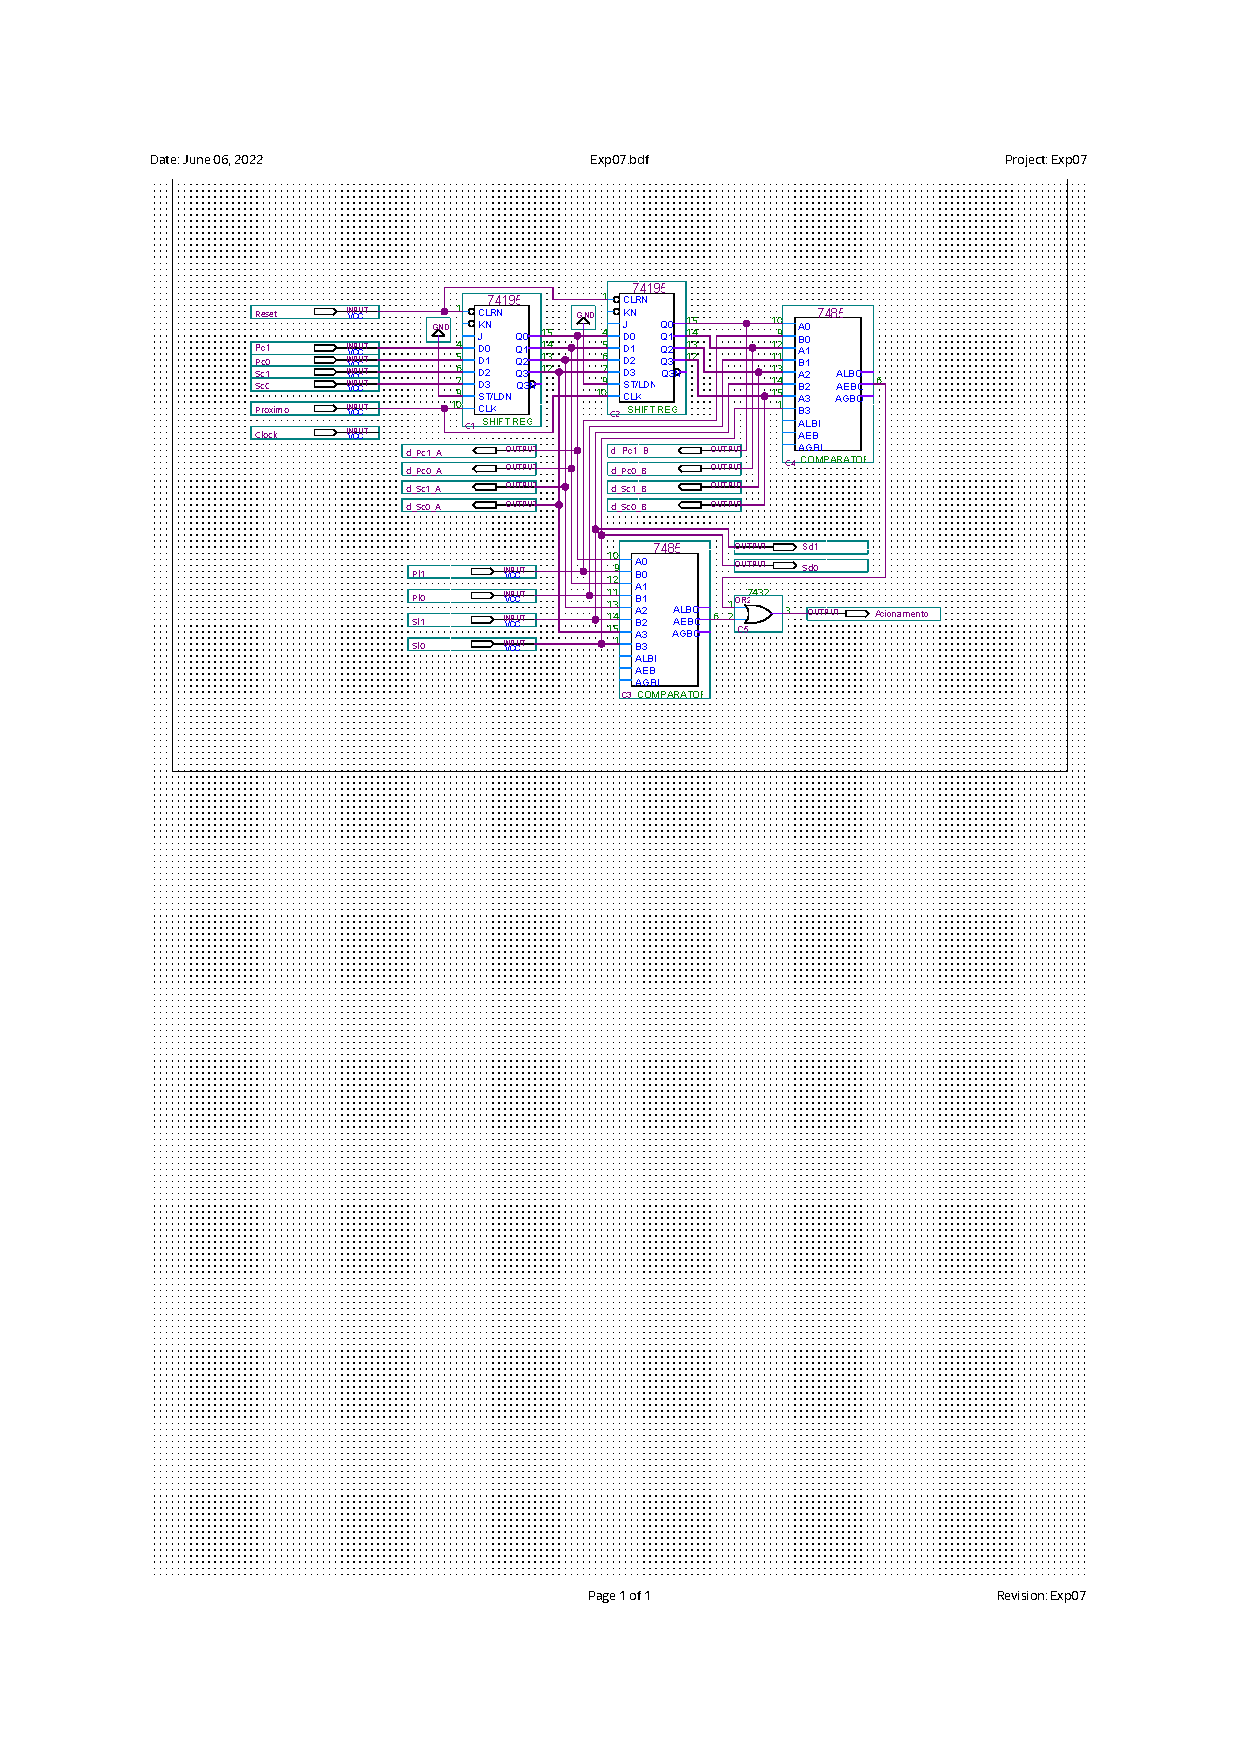
\includegraphics[width=\textwidth, trim={42mm, 175mm, 50mm, 47mm}, clip]{diagrama_logico.pdf}%
        }%
    }
    \caption{Diagrama lógico do fluxo de dados da esteira classificadora.}
    \label{fig:diagrama_logico}
\end{figure}

\subsubsection{Levantamento dos materiais necessários}
\label{sec:plan_materiais}

\begin{table}[!ht]
    \centering
    \caption{Unidades requeridas para cada CI}
    \label{tab:materiais}
    \doubleRuleSep
    \begin{tabular}{lllrr}
        \doubleTopRule
        Slot & Operação & CI & Un. Requeridas & Un. Disponíveis \\
        \midrule
        1 & Registrador & 74195 & 1 & 1\\
        2 & Registrador & 74195 & 1 & 1\\
        3 & Comparador & 7485 & 1 & 1\\
        4 & Comparador & 7485 & 1 & 1\\
        5 & OR2 & 7432 & 1 & 4\\
        \doubleBottomRule
    \end{tabular}
\end{table}

    Para garantir que o circuito projetado respeite as restrições de montagem, fizemos um levantamento dos recursos necessários para este circuito mostrado na Tabela \ref{tab:materiais}. Ela mostra a quantidade de unidades lógicas requeridas para cada CI utilizado. As especificações de cada CI foi obtido pelos respectivos \emph{datasheets}.

\subsubsection{Simulação}
\label{sec:plan_sim}
    A Fig. \ref{fig:carta_tempos} mostra a carta dos tempos obtida com a simulação do Fluxo de Dados. Essa simulação visa imitar uma situação na qual o operador da máquina inicialmente configura os prdutos e seus respectivos setores e logo em seguida passam todas as conbinações de produtos e setores para verificar se apenas os predutos e setores configurados forneceriam saída alta do circuito. 
    
    Como é possível ver na simulação, esses sinais mostram que o resultado esperado foi alcançado na simulação.

\begin{figure}[!ht]
    \centering
    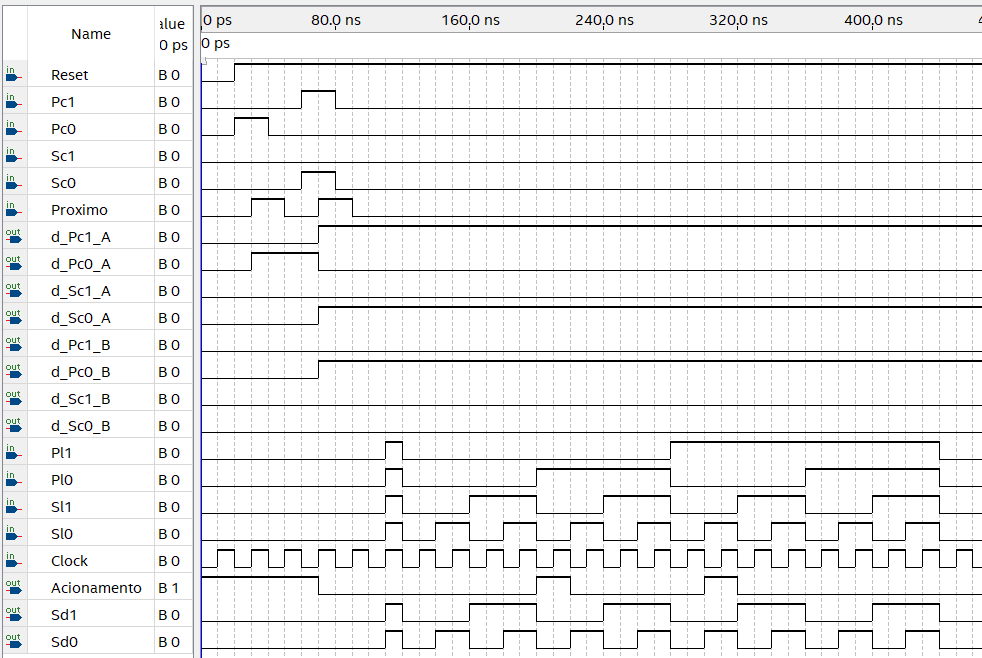
\includegraphics[width=\textwidth]{carta_tempos.png}
    \caption{Carta dos tempos para o circuito do fluxo de dados da Esteira Classificadora com sinias de entrada \texttt{Clock}, \texttt{Reset}, $Pc1$, $Pc0$, $Sc1$, $Sc0$, \texttt{Proximo}, $Pl1$, $Pl0$, $Sl1$ e $Sl0$, sinais de depuração $d\_Pc1\_A$, $d\_Pc0\_A$, $d\_Sc1\_A$, $d\_Sc0\_A$, $d\_Pc1\_B$, $d\_Pc0\_B$, $d\_Sc1\_B$, $d\_Sc0\_B$, e sinais de saída \texttt{Acionamento}, $Sd1$ e $Sd0$}
    \label{fig:carta_tempos}
\end{figure}

\newpage
\subsubsection{Metodologia de montagem e testes}
\label{sec:plan_ff_montagem}
O circuito será montado no painel de montagem e testado à medida que for montado. Incialmente, monta-se um registrador e um comparador, testa-se então o seu comportamento, logo em seguida monta-se os demais componentes. Após estar todo montado será avaliado com a tabela de testes (Tab. \ref{tab:tb_teste}).


\subsubsection{Tabela de Testes}

As Tabelas \ref{tab:tb_teste} e \ref{tab:tb_dep} são as tabelas de testes para os sinais de saída e depuração, respectivamente. 

\begin{table}[!ht]
    \centering
    \caption{Tabela de testes para o sinal de saída}
    \label{tab:tb_teste}
    \doubleRuleSep
    \begin{tabular}{*{14}{c}}
        \doubleTopRule
        \multicolumn{11}{c}{Entrada} & \multicolumn{3}{c}{Saída}\\
        \cmidrule(lr){1-11}\cmidrule(lr){12-14}
        Clk & Rst & $Pc_1$ & $Pc_0$ & $Sc_1$ & $Sc_0$ & Prox & $Pl_1$ & $Pl_0$ & $Sl_1$ & $Sl_0$ & Ac & $Sd_1$ & $Sd_0$\\
        \midrule
        \csvreader[head to column names, late after line=\\]{tb_teste.csv}{}%
        {\csvcoli & \csvcolii & \csvcoliii & \csvcoliv & \csvcolv & \csvcolvi & \csvcolvii & \csvcolviii & \csvcolix & \csvcolx & \csvcolxi & \csvcolxii & \csvcolxiii & \csvcolxiv} %& \csvcolxv & \csvcolxvi & \csvcolxvii & \csvcolxviii}%
        \doubleBottomRule
    \end{tabular}
\end{table}

\newpage
\begin{table}[!ht]
    \centering
    \caption{Tabela de testes para os sinais de depuração}
    \label{tab:tb_dep}
    \doubleRuleSep
    \begin{tabular}{*{17}{c}}
        \doubleTopRule
        \multicolumn{9}{c}{Entrada} & \multicolumn{8}{c}{Depuração}\\
        \cmidrule(lr){1-9}\cmidrule(lr){10-17}
        $Pc_1$ & $Pc_0$ & $Sc_1$ & $Sc_0$ & Prox & $Pl_1$ & $Pl_0$ & $Sl_1$ & $Sl_0$ & $Pc_1^A$ & $Pc_0^A$ & $Sc_1^A$ & $Sc_0^A$ & $Pc_1^B$ & $Pc_0^B$ & $Sc_1^B$ & $Sc_0^B$\\
        \midrule
        \csvreader[head to column names, late after line=\\]{dep.csv}{}%
        {\csvcoliii & \csvcoliv & \csvcolv & \csvcolvi & \csvcolvii & \csvcolviii & \csvcolix & \csvcolx & \csvcolxi & \csvcolxii & \csvcolxiii & \csvcolxiv & \csvcolxv & \csvcolxvi & \csvcolxvii & \csvcolxviii & \csvcolxix}%
        \doubleBottomRule
    \end{tabular}
\end{table}

\newpage
\section{Resultados}
    O circuito digital foi implementado com sucesso na placa de montagem. Ele apresentou os mesmos resultados que os obtidos nas simulações. A montagem do circuito pode ser visto na Fig. \ref{fig:montagem}.
    
\begin{figure}[!ht]
    \centering
    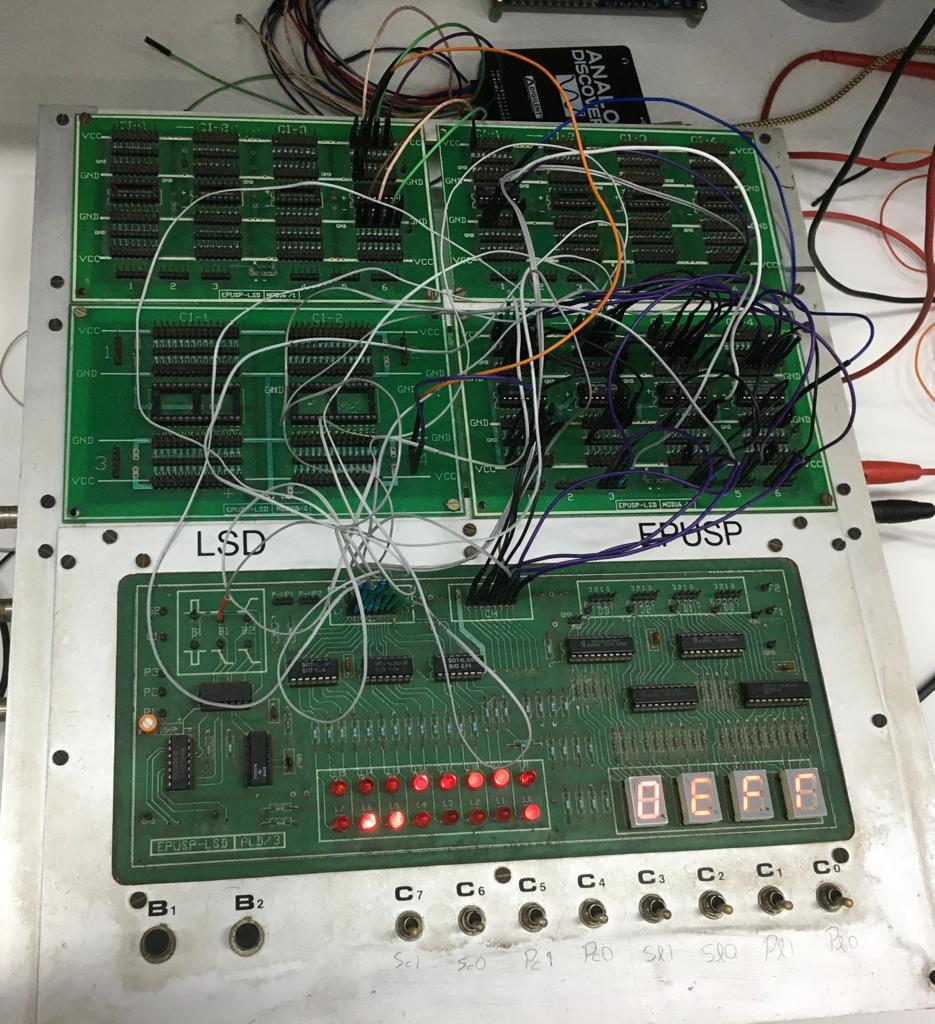
\includegraphics[width=\textwidth]{montagem.jpeg}
    \caption{Montagem do Fluxo de Dados do projeto da esteira classificadora de produtos.}
    \label{fig:montagem}
\end{figure}

\section{Desafio}
% Como desafio, foi proposto pelo professor, que fosse desenhado um diagrama de blocos da unidade de controle e do fluxo de dados com seus respectivos sinais de controle, entrada de dados e saída de dados. Para esse desafio, a dupla chegou no resultado que pode ser visto na Fig. \ref{fig:desafio}.

O próximo passo é introduzir uma unidade de controle ao circuito juntamente com o fluxo de dados projetado. Consideramos, agora, que o circuito possui dois modos de funcionamento: configuração e operação, que são controlados pelo sinal externo \emph{modo}. Adotamos a convenção de que o circuito entra em estado de configuração quando o sinal \emph{modo} está em nível lógico alto e em estado de operação quando o sinal \emph{modo} está em nível lógico baixo. Com esta escolha, o sinal \emph{enable} possui a expressão lógica $enable = modo \cdot proximo$. É o sinal \emph{enable} que controla a entrada \emph{proximo} do fluxo de dados, permitindo a configuração de um novo produto apenas se o circuito estiver em estado de configuração. O diagrama de blocos do  circuito descrito é mostrado na Fig. \ref{fig:desafio}.

    
\begin{figure}[!ht]
    \centering
    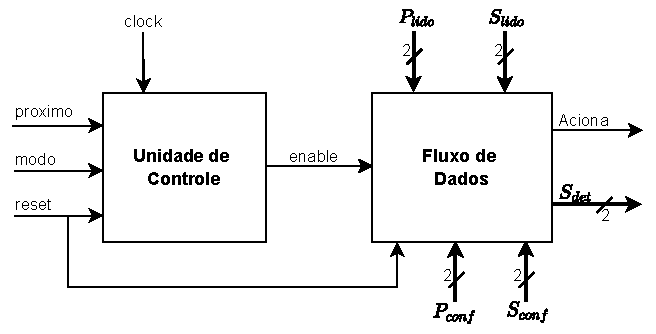
\includegraphics[width=0.9\textwidth]{blocos.pdf}
    \caption{Diagram de blocos da esteira classificadora incluindo a unidade de controle}
    \label{fig:desafio}
\end{figure}
    
\section{Conclusão}
    Com este experimento, pudemos projetar um Fluxo de dados de uma projeto de uma esteira classificadora de produtos. O desenvolvimento do fluxo de dados foi feito a partir do diagrama de blocos fornecido e da descrição de funcionamento da máquina. Durante a implantação não houve nenhuma alteração do planejamento e o circuito operou como planejado.
    
\horizonBackCover
\end{document}